\documentclass[border=10pt]{standalone}

\usepackage{tikz}
\usepackage{tikzsymbols}
\usetikzlibrary{calc,patterns,shapes.geometric}

\def\centerarc[#1](#2)(#3:#4:#5){\draw[#1] ($(#2)+({#5*cos(#3)},{#5*sin(#3)})$) arc (#3:#4:#5);}

\begin{document}
	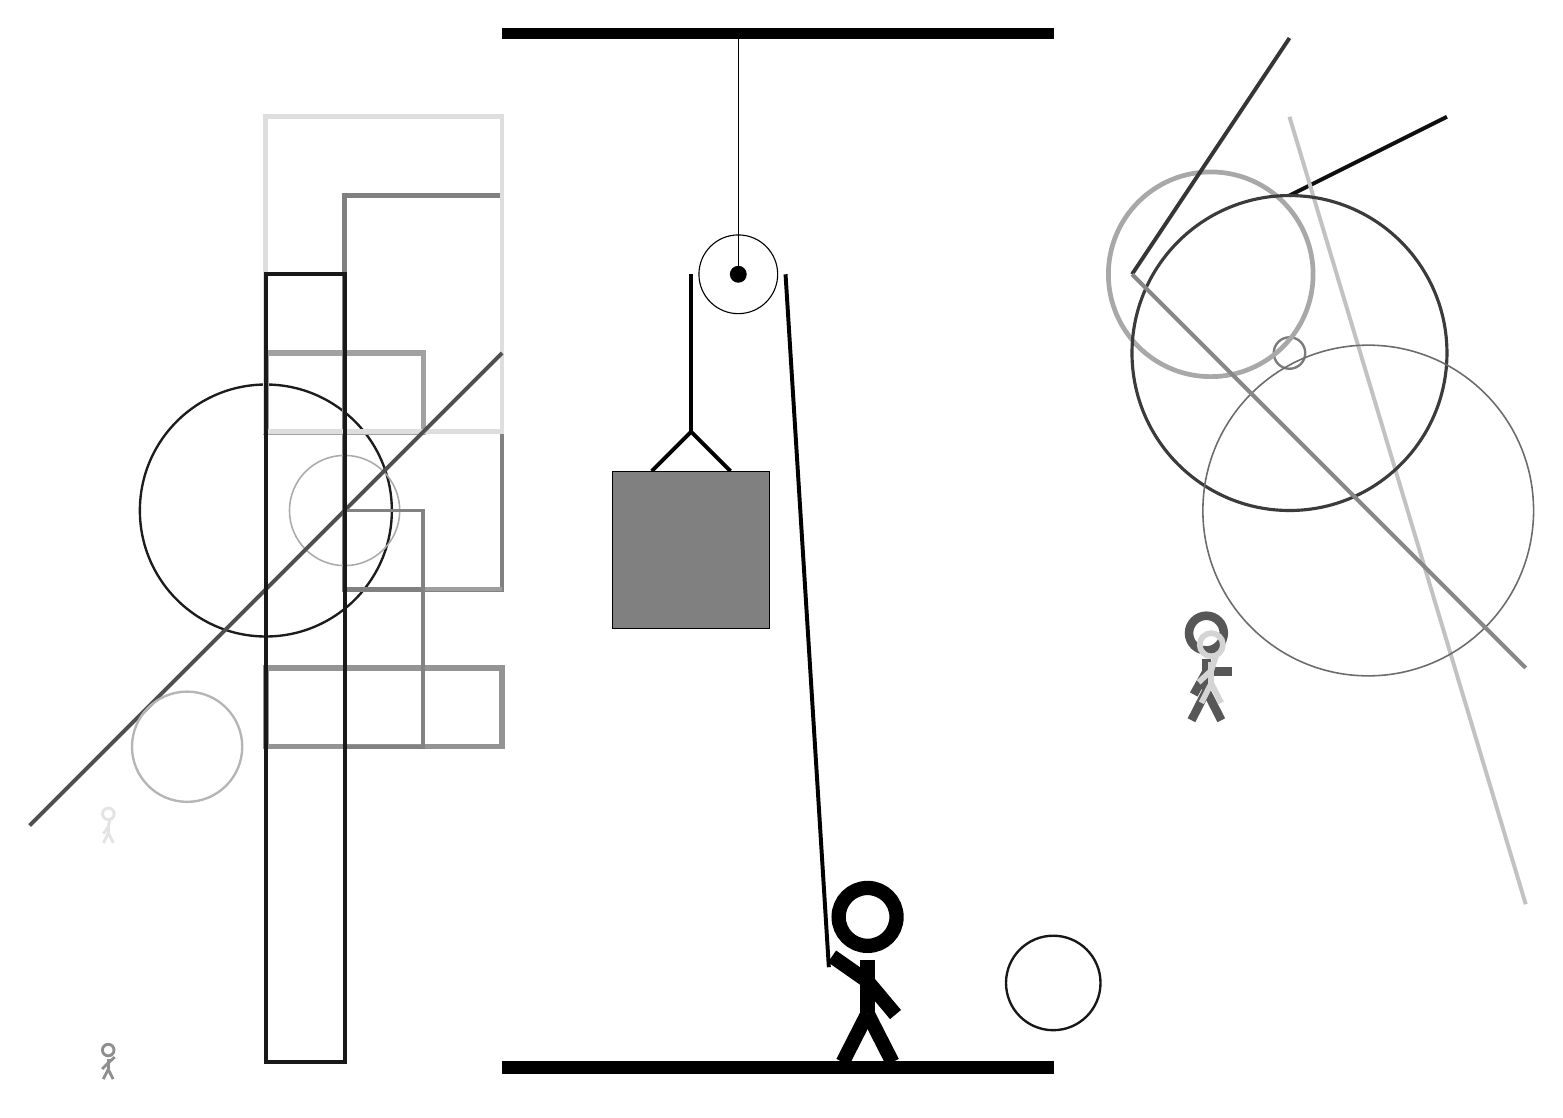
\begin{tikzpicture}
		%%%%% START %%%%%
		
		\draw[fill=black] (-2, 10) rectangle (5, 10.125);
		
		\draw (1, 7) circle (0.5);
		\draw[fill=black] (1, 7) circle (0.1);
		\draw (1, 10) -- (1, 7);
		
		\draw[line width=0.5mm] (-0.1, 4.5) -- (0.4, 5.0) -- (0.9, 4.5);
		\draw[fill=black!50] (-0.6, 4.5) rectangle (1.4, 2.5);
		
		\draw[line width=0.5mm, color=black!94](8, 8) -- (10, 9);
		
		\node[line width=0.7mm, color=black!44] at (-7, -3) {\Strichmaxerl[2][45][42]};
		\draw [line width=0.3mm, color=black!52](8, 6) circle (0.2);
		\draw [line width=0.3mm, color=black!89](-5, 4) circle (1.6);
		\node[line width=0.3mm, color=black!11] at (-7, 0) {\Strichmaxerl[2][54][77]};
		
		\draw[line width=0.7mm, color=black!42] (-2, 1) rectangle (-5, 2);
		\draw [line width=0.6mm, color=black!34](7, 7) circle (1.3);
		\draw[line width=0.5mm, color=black!24](8, 9) -- (11, -1);
		\draw[line width=0.5mm, color=black!79](6, 7) -- (8, 10);
		
		\node[line width=0.5mm, color=black!66] at (7, 2) {\Strichmaxerl[6][61][0]};
		\node[line width=0.2mm, color=black!17] at (7, 2) {\Strichmaxerl[4][43][72]};
		\draw[line width=0.7mm, color=black!37] (-3, 5) rectangle (-5, 6);
		\draw[line width=0.6mm, color=black!50] (-2, 8) rectangle (-4, 3);
		
		\draw [line width=0.2mm, color=black!33](-4, 4) circle (0.7);
		\draw [line width=0.3mm, color=black!91](5, -2) circle (0.6);
		\draw [line width=0.2mm, color=black!77](6, 4) circle (0.0);
		
		\draw [line width=0.4mm, color=black!77](8, 6) circle (2.0);
		\draw[line width=0.6mm, color=black!13] (-2, 5) rectangle (-5, 9);
		\draw[line width=0.5mm, color=black!69](-2, 6) -- (-8, 0);
		\draw [line width=0.2mm, color=black!58](9, 4) circle (2.1);
		\draw [line width=0.3mm, color=black!29](-6, 1) circle (0.7);
		\draw[line width=0.5mm, color=black!47](6, 7) -- (11, 2);
		
		\draw[line width=0.5mm, color=black!38] (-3, 3) rectangle (-2, 3);
		\draw[line width=0.5mm, color=black!49] (-4, 4) rectangle (-3, 1);
		\draw[line width=0.5mm, color=black!90] (-4, -3) rectangle (-5, 7);
		
		
		\draw[line width=0.5mm] (0.4, 7) -- (0.4, 5.0);
		\centerarc[line width=0.5mm](1, 7)(0:180:0.6);
		\draw[line width=0.5mm](1.6, 7) -- (2.15, -1.8);
		
		\node at (2.6, -1.9) {\Strichmaxerl[10][-35][-50]};
		
		\draw[fill=black] (-2, -3) rectangle (5, -3.15);
		
		%%%%% END %%%%%
	\end{tikzpicture}
\end{document}